\chapter{Diseño hardware}
\label{chap:hard}
\graphicspath{{hard/figs/}{hard/figs/}}

%******************************************************************************************************************************************************


\section{Herramientas de diseño}

Para la implementación hardware del sistema se ha utilizado la herramienta \textit{Altium Desinger}: Altium es un potente entorno de desarrollo que incluye todas las herramientas necesarias durante el proceso de diseño, prueba y fabricación de un prototipo hardware.

\begin{figure}[hbt!]
	\centering
	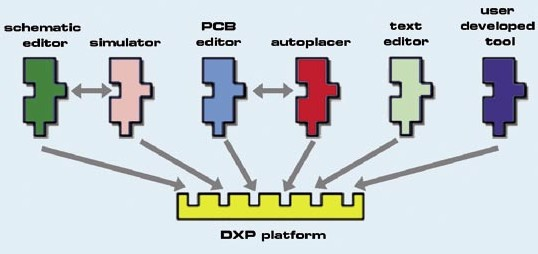
\includegraphics[width=0.7\linewidth]{altium.jpg}
	\caption{Componentes de Altium DPX}
	\label{fig::altium}
\end{figure}

Altium es uno de los softwares de diseño hardware más utilizado actualmente por la industria, además cuenta con una gran cantidad de documentación, la cual facilita en uso y el aprendizaje. Todas estas ventajas han hecho que Altium sea la herramienta elegida para desarrollar este apartado del TFG.

Con Altium se han llevado a cabo las tareas de diseño de esquematicos, creación de componentes y footprints, diseño y rutado de la tarjeta y la generación de los ficheros de fabricación. Aunque Altium es un software propietario con un coste elevado, para la realización de los prototipos se han utilizado licencias de prueba del software. 



\section{Elección del hardware}
	\subsection{Integrado CMWX1ZZABZ}
	
	El integrado CMWX1ZZABZ es un módulo diseñado por \textit{Murata}, que incorpora un microcontrolador STM32L0 y un tranceptor de radio SX1276 en el mismo chip. La forma en la que se encuentran conectados ambos módulo en el chip, se resume en la figura  \ref{fig:CMWX1ZZABZ} .
	
	
	\begin{figure}[hbt!]
		\centering
		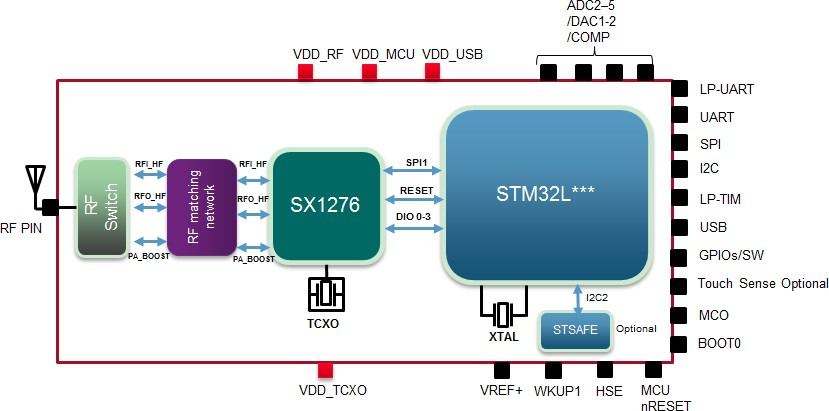
\includegraphics[width = \linewidth]{MurataMCU.jpg}
		\caption{Esquema de bloques del chip CMWX1ZZABZ}
		\label{fig:CMWX1ZZABZ}
	\end{figure}
	
	La principal ventaja de este chip, es que reduce en gran medida en espacio utilizado, reduciendo el tamaño final de la tarjeta  y simplificando las conexiones.
	\subsubsection{Microcontrolador STM32L072}
	
	El STM32l072, es un microcontrolador de ultrabajo consumo, diseñado por la empresa \textit{STMicrocontrollers}. Cuenta con una arquitectura de Arm Cortex-M0+ de 32 bits funcionando a 32 MHz, además 192 KB de memoria flash, 6 KB de memoria de datos y 20 KB de memoria RAM. Este microcontralador tiene un amplio abanico de perifericos como SPI, $I^2C$, USART, USB, ADC, USB entre otros. 
	\paragraph{}	
	Lo más destacable de este microcontrolador es ultra-bajo consumo, y sus diferentes modos de funcionamiento, los cuales podemos ver resumido en la figura \ref{fig::powerMCU}. El bajo consumo y altas prestaciones de este chip, lo hacen ideal para este proyecto.
	
	\begin{figure}[hbt!]
		\centering
		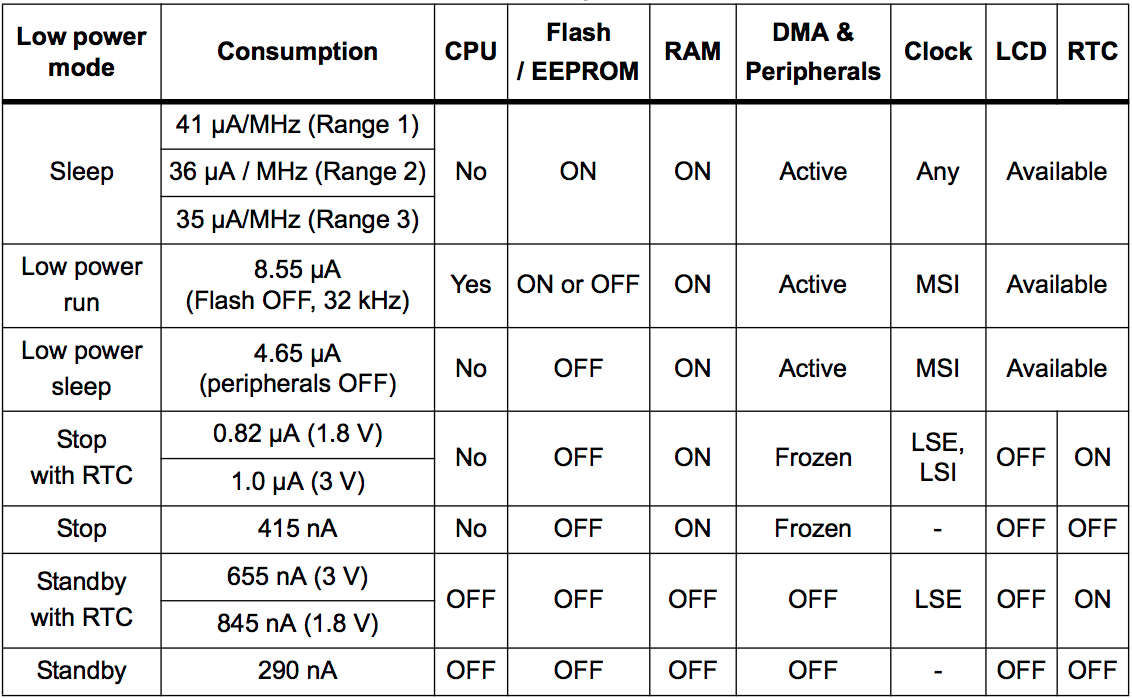
\includegraphics[width = 0.7\linewidth]{powerMCU.png}
		\caption{Consumo y modos de funcionamiento del microcontrolador STM32L072}
		\label{fig::powerMCU}
	\end{figure}
	
	\subsubsection{Transceptor SX1276}
	
	El SX1276 es un tranceptor de radio, diseñado por \textit{Semtech}, preparado para trabajar con la modulación lora en sistemas de largo alcance y bajo consumo. También puede funcionar como modulador FSK/OOK.
	
	\begin{figure}[hbt!]
		\centering
		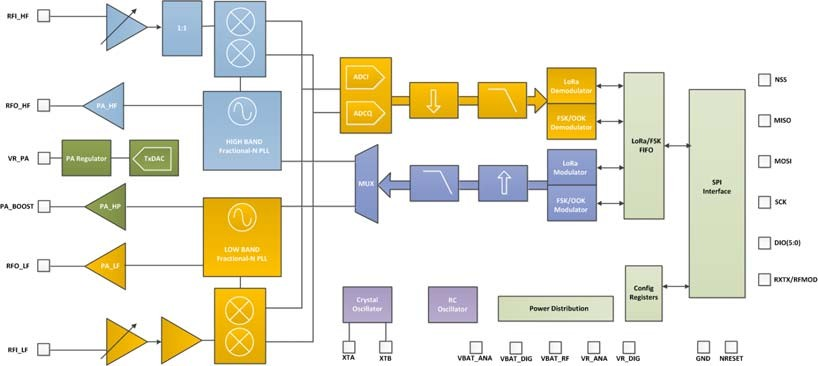
\includegraphics[width = 0.7\linewidth]{sx1276.jpg}
		\caption{Esquema de bloques de la familia de tranceptores SX127x}
	\end{figure}
	
	
	Se carateriza por trabajar en un rango de frecuencias desde 137 MHz hasta los 1020 MHz, con un \textit{"spreading factor"} o factor de enchanchado entre 6 y 12, un ancho de banda entr 7.5 KHz y 500 KHz y una sensibilidad entre -111 dBm y -148 dBm. Con todo esto, consigue velocidades binarias efectivas ente los 18 bps y los 37.5 Kbps.
	\paragraph{}
	Por otro lado, el trasmisor tiene un consumo típico de 10.8 mA en recepción, de entre 20 mA  y 120 mA en recepción (dependiento de la configuración) y un consumo típoco en modo \textit{sleep} de 0.2 uA.
	
	
	\subsection{Conversor analógico/digital AD7194}
	
	El AD7194 es un conversor analógico/digital de bajo ruido diseñado para aplicaciones de alta presición. Creado por \textit{Analog}, posee 16 canales de entrada analógicos, una resolución de 24 bits, un reloj interno de 4.92 MHz y un amplificador de entrada de ganacia programable. La comuicación se hace a través de la interfaz SPI del ADC y el SPI-2 del microcontrolador.
	
	\begin{figure}[htb!]
		\centering
		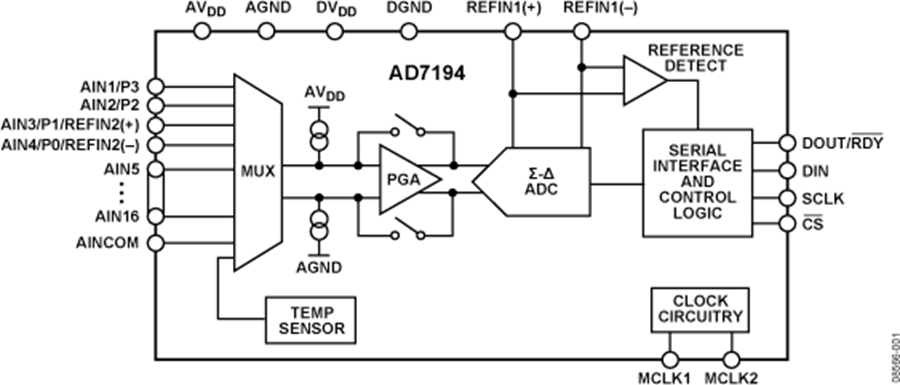
\includegraphics[width=0.7\linewidth]{AD7194.png}
		\caption{Diagrama funcional del AD7194}
	\end{figure}
	
	Entre sus opciones de configuración, permite la utilización de filtros digitales programables, rechazo de las bandas de 50 Hz y 60 Hz y la utilización de sus canales en modo diferencial (en cualquier configuración) o en modo pseudo-diferencial (tomando como canal negativo GND). Otra de las característica decisivas, es su consumo,  que varia entre los 0.85 mA y los 5.3 mA en función de la ganancia de entrada elegida.
	
	\paragraph{}
	La motivación de usar este ADC, es su aplicación: La medida de termopares. En esta aplicación, se hace necesario una gran presición (las variaciones de tensión en los termopares es muy pequeña) y el bajo ruido de cuantificación. Además, al tener 16 de canales, se pueden utilizar un mayor número de termopares.
	
	
	\subsection{Sensor de temperatura MCP9808T}
	
	El MCP9808T es un sensor de temperatura digital, que permite medir termperaturas entre -20 ºC y 100 ºC con una presición de  $\pm 0.25 ºC$. Entre su características destaca su comunicación a través de $I^2C$, sus diferentes modos de operación y su bajo consumo, el cual ronda los 200 uA en funcionamiento.
	
	Su finalidad en el proyecto, será aproximar la temperatura de unión de los conectores a los termopares, la cual es necesaria para realizar una correcta medida (la union de cobre + estaño de los conectores genera una diferencia de potencial parácita que influye en las medidas).
	
	\subsection{Componentes activos}
	
	
	\begin{itemize}
		\item \textbf{Regulador TLV755P: }
		
		\item \textbf{Regulador AD1582BRTZ: }
		
		\item \textbf{Operacional MCP6001T: }
	\end{itemize}
	
	\subsection{Componentes pasivos}
	
	
\section{Diseño las tarjetas}

	\subsection{Fase 1: nodo básico} 
	
		En esta parte se diseñará un nodo general, sin aplicación específica que contendrá lo necesario para un correcto funcionamiento del microcontrolador y la radio. Se procurará minimizar el tamaño y número de componentes.
		
		\subsubsection{Esquemáticos}
		
		\subsubsection{Layout}
		
	\subsection{Fase 2: Tarjeta de expación}
	
	En esta fase se diseñará 
		\subsubsection{Esquemáticos}
		
		\subsubsection{Layout}
		
\section{Lista de componentes}
	
\section{Fabricación y montaje}



